\section{Evaluation}
\label{sec:evaluation}
This section describes the evaluation of the proposed design.
Section \ref{sec:design} introduces the design of the experiment to evaluate the system. 
Section \ref{sec:measurements} identifies the measurements in the system for the experiment.
Section \ref{sec:pilot_test} describes the pilot test used to compute the number of replication in the actual evaluation. 
Section \ref{sec:analysis} presents the analysis of the results from the experiment. 


\subsection{Experiment design}
\label{sec:design}
The performance of the system will be experimented, where the main goal of the experiment is to investigate the message latency between two services which are inferred between brokers. Thereby, the subsequent goals are accomplishing efficient and effective collaboration and communication between services.
The following hypothesis has been defined for the quality attribute, which will be further investigated with the experiment:
\textit{“Message latency between two independent services is lower if the communication is inferred between one broker instead of two, and should at maximum have one second of lead time.”}
With the stated hypothesis the relations between message latency and message broker will be investigated, and the metrics to be generated will either approve or disapprove the hypothesis. It is expected that the latency will be lower with one broker; however, it would minimize the plug and play capabilities of the architecture proposed for the project.

\subsection{Measurements}
\label{sec:measurements}
The primary metric to be accounted for is the timeliness of data exchange for end-to-end latency between services utilised by the overall production system. This would mean that the amount of time it takes for data to be exchanged between two respective and independent services within the system will be investigated. This is essential, as it would provide great knowledge in finding out the latency when using multiple brokers, and if it is suitable for the current architectural setup. 
\subsubsection{Test scenarios}
To accommodate a proper test scenario that would consider the design of the experiment, the scenario is to test end-to-end latency between two services. First by explicitly assigning timestamp values on every produced event - or more specifically a particular topic that is used between the production floor and all the way to the designated warehouse. This would mean to measure the time it takes for a message to be produced by one independent service, to then be consumed by another service.

An example of how to do the calculations is by subtracting the timestamp of the message when produced, to when it gets consumed, and visualise through different graphical methods. This could be done by utilising line charts to show how latency changes over time.

\subsection{Pilot test}
\label{sec:pilot_test}
The context of doing the experimentation will be in a university setting, through a simulated “toy model” for the validation of the quality attribute. Various utilities will be utilised such as Docker Desktop, Docker Compose, Kafka Ecosystem, VScode, different programming languages and databases, as well as communication channels. 

Figure \ref{fig:experiment-diagram} represents the architecture of the system. The Robot arms and Warehouse service, which has been marked with red, are the two services that the experiments will be conducted between.

\begin{figure}[!htb]
    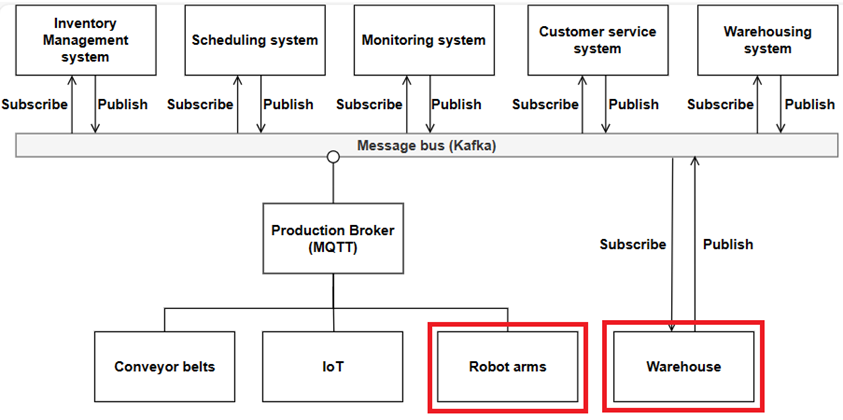
\includegraphics[width=250pt]{images/experiment-diagram.png}
    \caption{Deployment diagram with the two services marked which the experiment will be conducted between.}
    \label{fig:experiment-diagram}
\end{figure}

\subsubsection{Test objective}
The first objective the Warehouse service, that is coupled to a global Kafka broker, consumes events produced by the Robot arms service which is coupled to a MQTT broker due to its hardware level. This means producing and consuming events by the Warehouse service, is transferred between two brokers and the latency metrics are gathered through this setup. For the second objective, the Warehouse service is coupled directly to the MQTT broker which it will consume the events through, and latency metrics will be gathered through this direct setup.
About one second for real-time latency is required as the recommended interval is around half a second. This would increase the chance of success. Additionally, it is preferred that the timeliness of data gathered to be generated through the utilisation of the virtual machines provided by University of Southern Denmark (SDU).

All the data is stored on an external PostgreSQL also coupled to the architecture, but more specifically, to the SCMS primary system consolidating multiple different services. When doing the test scenario, the amount of data to be gathered will be taken into consideration. The procedure for this experiment is to start from small snippets of batch data, and if more is required the data generation will be extended. This would minimize the risk of overdoing the metric generation since small batches of data could be sufficient to approve or disapprove the hypothesis.  

\subsection{Analysis}
\label{sec:analysis}
The results of the above mentioned experiments were stored in a PostgreSQL database. The table was structured with an id, a timestamp when the event was produced, and a timestamp when it was consumed. Figure \ref{fig:timestamp-data} showcases a sample of the collected data in the database. 
\begin{figure}[h]
    \centering
    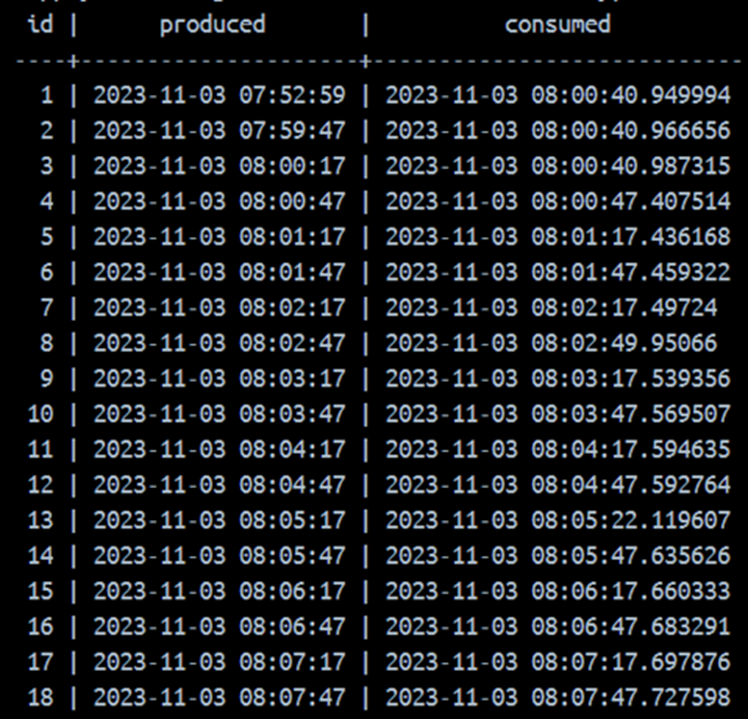
\includegraphics[width=190pt]{images/timestamp-data.png}
    \caption{Database structure, with id, produced and consumed columns}
    \label{fig:timestamp-data}
\end{figure}

From the collected data a Python script was developed in order to display data in the most effective visual presentation as possible. A line chart was chosen as the visualisation representation where the x-axis was the timestamps for each production cycle, and the y-axis was the time difference in seconds. The line chart was able to describe and examine the collected data and visually present if there were any outliers in the data.
The primary metric was the timeliness of data exchange for end-to-end latency between services of the overall system. The aim was to investigate the latency when utilising multiple brokers, whereas figure \ref{fig:linechart1} visualizes the first scenario by first producing an MQTT event, sending the event through the MQTT broker to Kafka and then to be consumed by the warehouse.
\begin{figure}[h]
    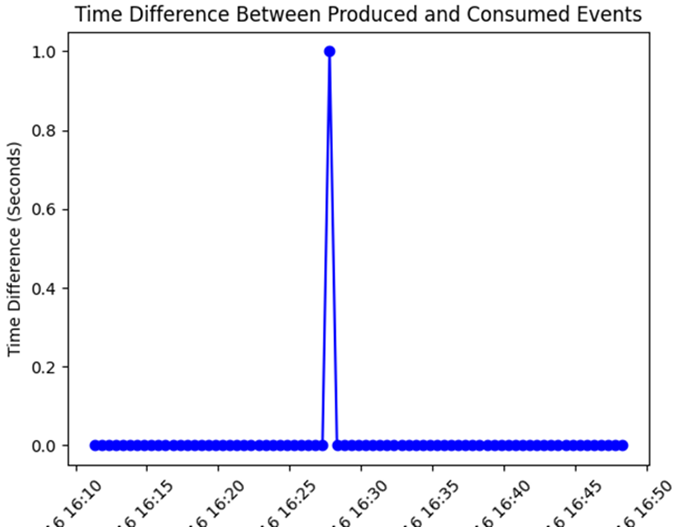
\includegraphics[width=195pt]{images/linechart1.png}
    \centering
    \caption{Line chart: Time difference with MQTT and Kafka}
    \label{fig:linechart1}
\end{figure}

The data point in the line chart describes a successful production cycle from the warehouse. The experiment was done over three hours where all relevant data was collected. The line chart displays a snippet within a 40 minute window, where it was shown that almost every data point is below one second, except one outlier. The outlier presents that the difference is one second which could be interfered with external factors. When exploring the line charts from the three hour experiment, it was shown that the other outliers was occurring on the same specific interval. This could be an indication of when the warehouse is loading for a new production cycle.
The second scenario was with a different procedure where the Kafka broker was not utilized. In this scenarious an MQTT event was produced by the production floor and then consumed by the warehouse directly through the MQTT broker.
Figure \ref{fig:linechart2} has same unit scale on both the x-axis and the y-axis. The data was collected with the same premises as the first scenario.
\begin{figure}[h]
    \centering
    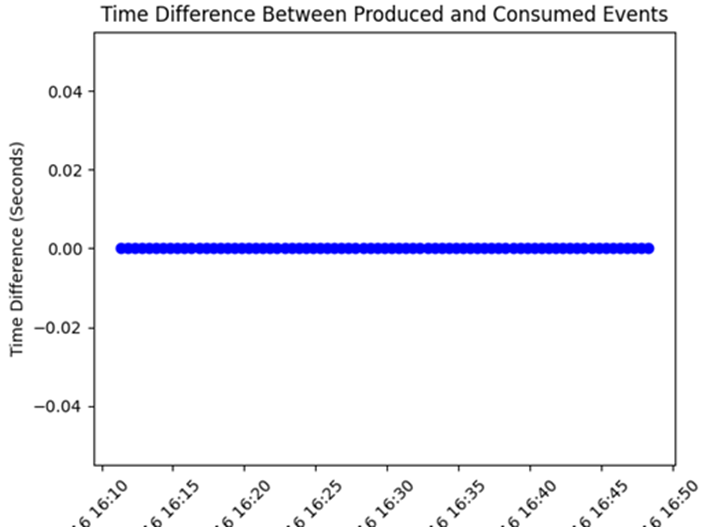
\includegraphics[width=195pt]{images/linechart2.png}
    \caption{Line chart: Time difference with only MQTT}
    \label{fig:linechart2}
\end{figure}

As seen on the line chart every data point is below one second and no outliers are present, which means that this experiment scenario was executed where nothing interfered.
After the experiment was done, the collected data in the database were extracted and the mean time was calculated to visualize the time difference at a very low level. As seen in Figure \ref{fig:meanovertime} the mean time for Kafka is high at the beginning of the experiment and then it is exponentially decreasing. Kafka nearly approaches the same level as MQTT which could indicate that Kafka runs better when it has been running for a while.
\begin{figure}[h]
    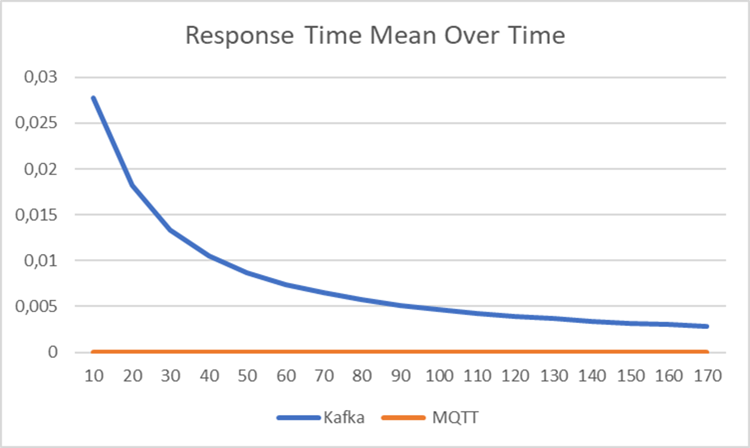
\includegraphics[width=220pt]{images/meanovertime.png}
    \centering
    \caption{Line chart which visualises the mean of the response time }
    \label{fig:meanovertime}
\end{figure}
\newpage
The collected results were presented as a line chart for both scenarios. The hypothesis was defined as \textit{“Message latency between two independent services is lower if the communication is inferred between one broker instead of two and should at maximum have one second of lead time“}. The results of both line charts confirms that the defined hypothesis was true, because of the first scenario where two brokers were utilised had a higher message latency than the second scenario. The mean time of the message latency of both scenarios showcased that both were under one second as seen in figure \ref{fig:meanovertime}. 

Of the experiment executed it was confirmed that when utilising two message brokers, there would be a higher message latency as seen in figure \ref{fig:meanovertime}. The reasoning behind why MQTT and a Kafka broker were utilised, was to ensure if the MQTT broker faulted, the Kafka broker which by default has a persistent message queue, would ensure that messages would not be lost\cite{docsKafka}. The time difference of both experiments are trivial whereas fault-tolerance is prioritised higher due to the minor timeliness difference.

The performance of both scenarios was almost the same which indicated that the current architectural design is optimal and complies with the stated requirements. Furthermore, each service was deployed in a Docker container, which makes it possible to ensure that every service would be replicated to ensure resilience. 